\chapter{全景漫游的信息架构}

用户在进行全景漫游时与场景进行交互,本质上是于场景的构成信息进行交互。简单的信息不需要组织,直接呈现给用户即可展示其内容。但当信息的复杂程度超过人所能同时认知的数量时,信息量过载会造成理解效率的急剧下降。信息架构是对某一类信息进行统筹、安排、规划等处理的方法,它决定了信息以何种形式展现给使用信息的人。信息架构的形式有很多种,常见的类似于组织机构的部门职务构成,以层级作为架构的主体形式,如图\ref{fig:structure}。其核心思想是同一职责或功能的内容进行归并分类,也就是人们常说的分类法。信息架构的形式随着应用情景的改变而做出调整,特别是根据使用信息的用户、信息的内容和信息的载体设备而综合分析。

\begin{figure}[htp]
\centering
\fbox{
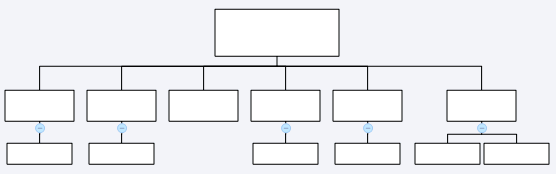
\includegraphics[width=.5\textwidth]{structure}
}
\caption{信息架构的常见组织形式}
\label{fig:structure}
\end{figure}


在全景漫游中,信息的呈现形式与数量与一般电子屏幕界面有着很大的差异,在一般人机界面上所适用的信息架构难以满足全景漫游的需要,故需要针对全景漫游所提供的使用场景,根据信息量的多寡、新旧、轻重进行划分,分主次、先后、缓急地进行有规划的呈现。

全景漫游的信息交互有可视化界面、可配戴设备的操作以及语音指令等多种实现形式,本章所涉及内容主要为可视化交互这种形式,辅以其他交互形式作为参照。以可视化交互作为信息架构的主线,从而引导用户在探索发现中认识并使用全景漫游系统。

\section{信息的组织形式}
可视化图形化人机界面即 GUI 界面由来已久,而最早的计算机则是需要科学家通过输入带孔纸带,计算机通过读取纸带上的小孔获取输入信息来进行运算,现今计算机用户甚至连 70~80 年代常见的命令行界面都未曾见过,如图\ref{fig:gui&cli}。

\begin{figure}[htp]
\centering
\fbox{
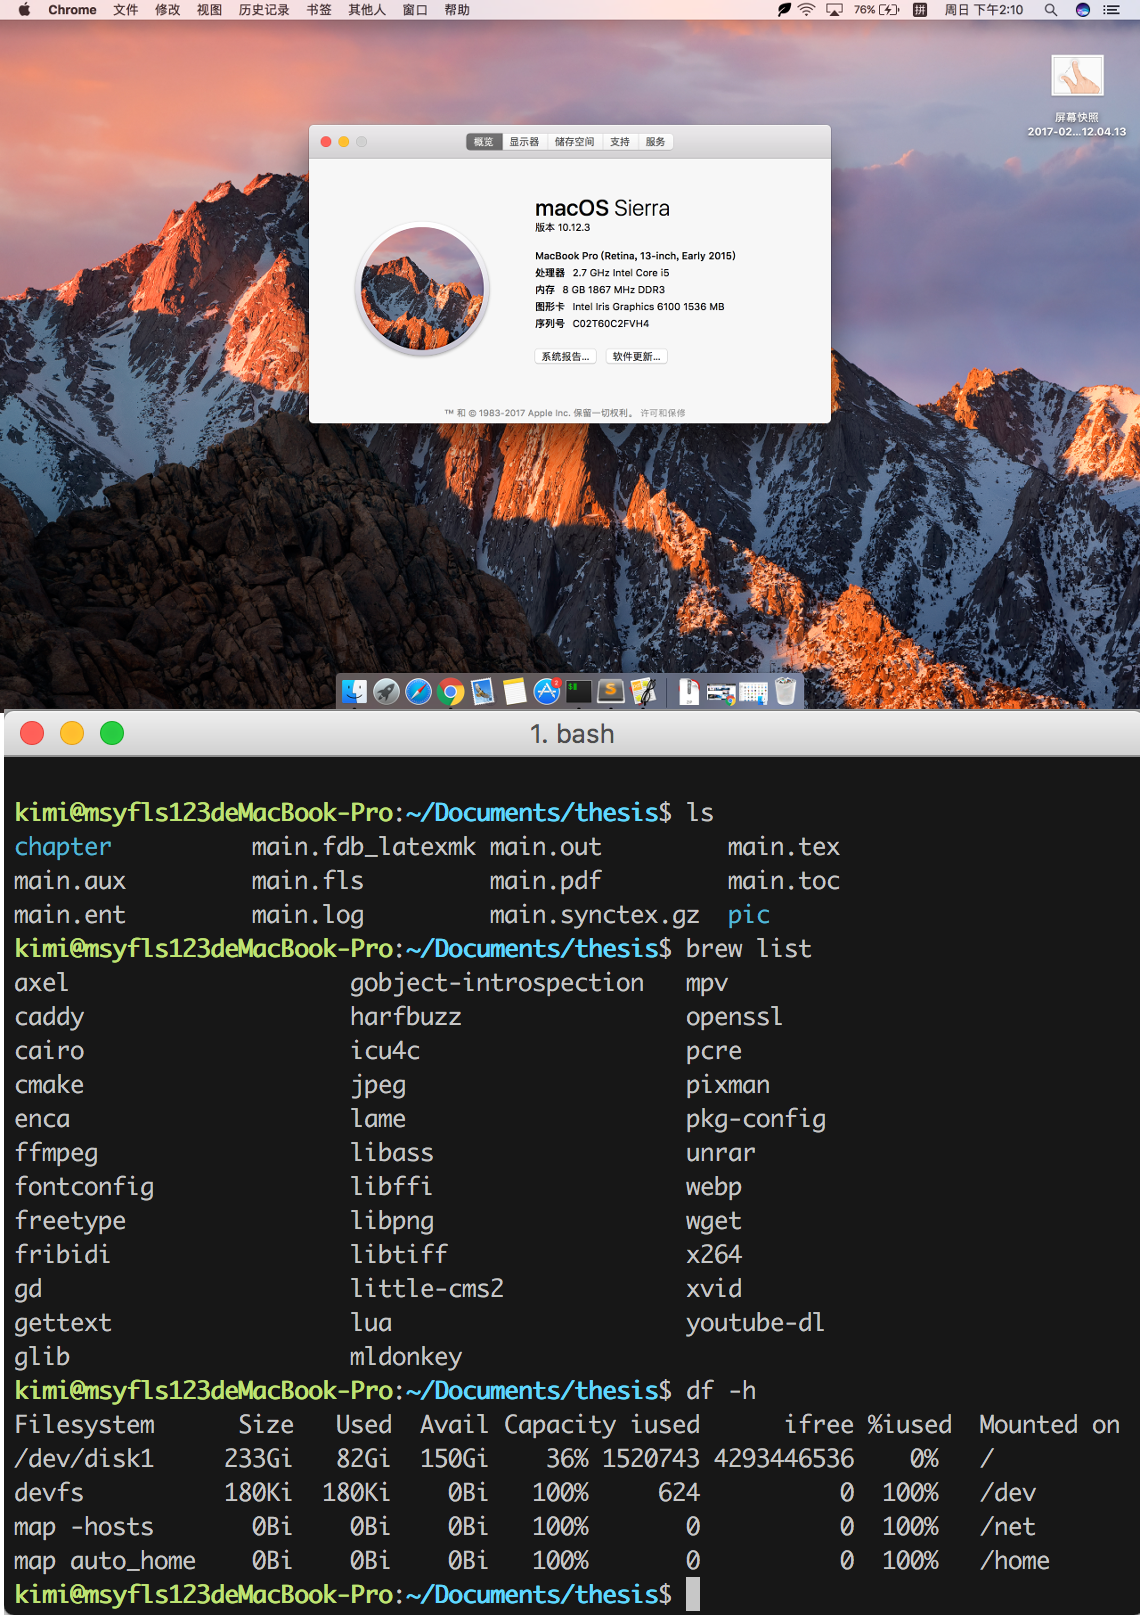
\includegraphics[width=.5\textwidth]{gui&cli}
}
\caption{图形化人机界面与命令行界面}
\label{fig:gui&cli}
\end{figure}

从命令行程序到图形化人机界面,用户获得的信息变得更多,但输入信息却减少了很多\endnote{Marchionini G, Brunk B. Toward a General Relation Browser: A GUI for Information Architects[J]. Journal of Digital Information, 2003, 4:2003.}。无数复杂的程序逻辑隐藏在一次又一次的鼠标点击或是手指点按后面,用户已经不是当年那群使用纸带操作计算机的科学家了。换而言之,用户无法准确记住那么多复杂的计算机命令,更不用提理解计算机内部的程序逻辑,他们只用理解计算机可以提供给他们的功能,例如通过点击某个按钮而无须记住类似“:w”这样的程序命令即可保存文件,并善加利用即可\endnote{杨明浩,陶建华,李昊,巢林林. 面向自然交互的多通道人机对话系统[J]. 计算机科学,2014,(10):12-18+35.}。

而图形化人机界面毕竟信息量相比与命令行界面信息量多出好几个数量级,例如一个全屏 Shell 窗口的信息量不会超过 500 字节,但是一个屏幕却有高达 $1920\times1080=2073600$ 个像素,而且图形化人机界面的信息变化效率高,可以用来表现视频动画等信息,其信息复杂度又提高了很多。

综上所述,在图形化人机界面时代随着信息爆炸而造成的信息过载(即信息的处理反馈速度低于信息生产的增长速度
,而造成信息沉积)促使信息界面的设计制作者需从信息架构的角度出发,减少冗余信息,整理信息的分布情况以使用户能更直观高效地获取使用信息\endnote{Beath C, Becerra-Fernandez I, Ross J, et al. Finding value in the information explosion[J]. Mit Sloan Management Review, 2012, 53(4):18-20.}。

下文将从信息模型、功能模型两条主线出发,探究全景漫游中可视化交互的可行技术路线,并结合相关理论尝试总结出部分经过实践检验或因技术选择而必然选用的功能模块,以供设计参考。


\section{全景漫游的信息模型}

全景漫游按形式可类比成游乐园,用户就像游客一样在场景中漫游,由此可以大致描绘出全景漫游的整体信息结构,如图\ref{fig:park}。这种假象的设计可以将使用者置于一种需求和环境相匹配的使用情景中,使用者可以借鉴平时游玩游乐场所积累的记忆,从场景中找寻到熟悉的“场所”以完成体验的过程。这种模式能够尽可能减少乃至消除用户对踏足陌生环境的恐惧感,人的行动预期也可以被规划在场景的设计中。

\begin{figure}[htp]
\centering
\fbox{
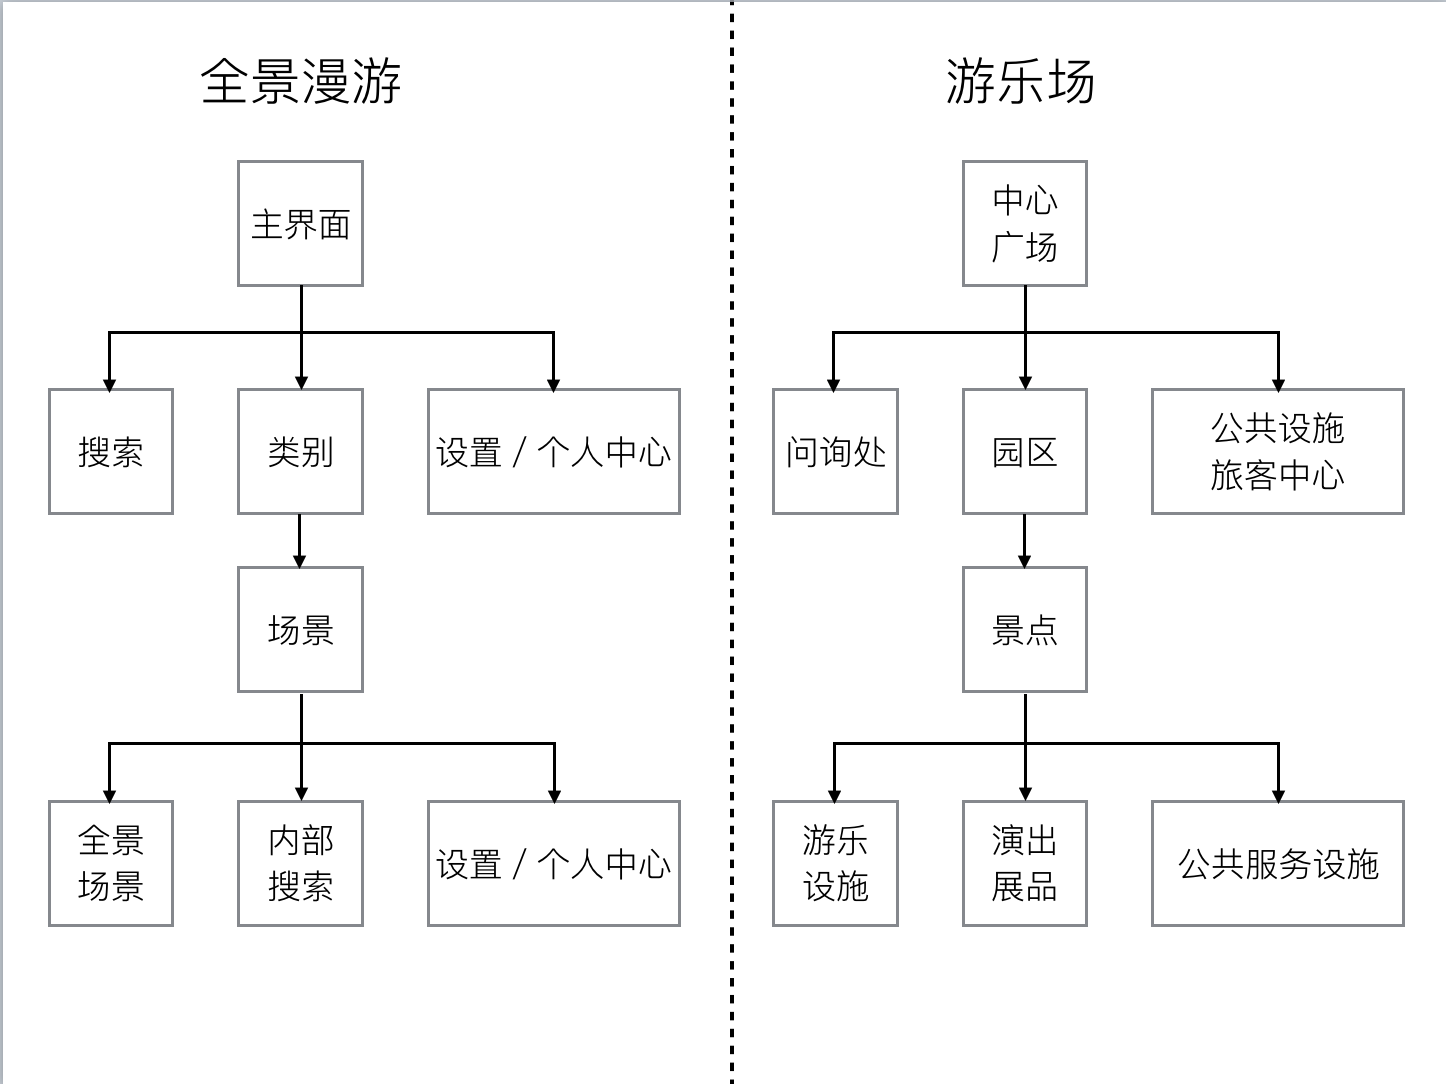
\includegraphics[width=.7\textwidth]{park}
}
\caption{全景漫游与游乐场的信息(组织)结构示意}
\label{fig:park}
\end{figure}

\subsection{信息架构组织形式}
信息架构的组织形式多样,一般而言可分为:自顶向下、自底向上和不可见的这三种形式。当前数以亿计的网站、应用和系统的信息架构都可以用它们来概括\endnote{罗森菲尔德, 莫尔维莱, 阿朗戈,等. 信息架构:超越Web设计[M]. 电子工业出版社, 2016.}。

自顶向下的信息架构是通常网页所采用的形式,其核心思想是用户已经有了一个需求概念和一个立足点(比如网站的首页),用户从首页出发,通过浏览展现的各种信息选择与自己的需求最为匹配的那个进行浏览(通常是进入下一个页面),然后在下一页面继续重复上述步骤直至找到自己所需的信息。自顶向下的信息架构非常清晰,所有类别目录都被呈现在用户面前,用户只需明确自己的需求就一定能找到“最接近”的那个页面\endnote{Larson K, Czerwinski M. Web page design: implications of memory, structure and scent for information retrieval[C]// Proceeding of the CHI '98 Conference on Human Factors in Computing Systems, Los Angeles, California, Usa, April. DBLP, 1998:25-32.}。但缺点是层级嵌套过深时容易使用户丧失进一步浏览的冲动,而往往此时离最后的页面只差一步之遥。自顶而下的信息层级以不超过三级为宜,在全景漫游中,“主界面-类别-场景”的层级刚好是三级,所以大部分导航类的场景(页面)采用这种信息架构是可行的。

自底向上的信息架构主要应用于服务于单个目的的应用中,主要通过建立事物间的联系来帮助用户在条目间切换。维基百科就是一个很好的例子,每一个词条都有众多相关链接指向其他的百科页面,通过不同的页面联结就构成了完整的知识体系。这种联系的方式也是现代搜索引擎排序的方式,即通过互相引用的计数来判断一个信息的权重,引用计数越高说明这条信息的真实性和准确性越高。全景漫游中单个场景的设计中可应用这种自底向上信息架构,例如在某个著名景点的全景漫游中,在浏览至某壁画前时通过点击其上的热点按钮,可以弹出关于该壁画的相关信息(如图\ref{fig:dunhuang}),这种信息代入方式相比传统的图文模式更容易使人沉浸于情景中,寓教于乐的效果更为理想。

\begin{figure}[htp]
\centering
\fbox{
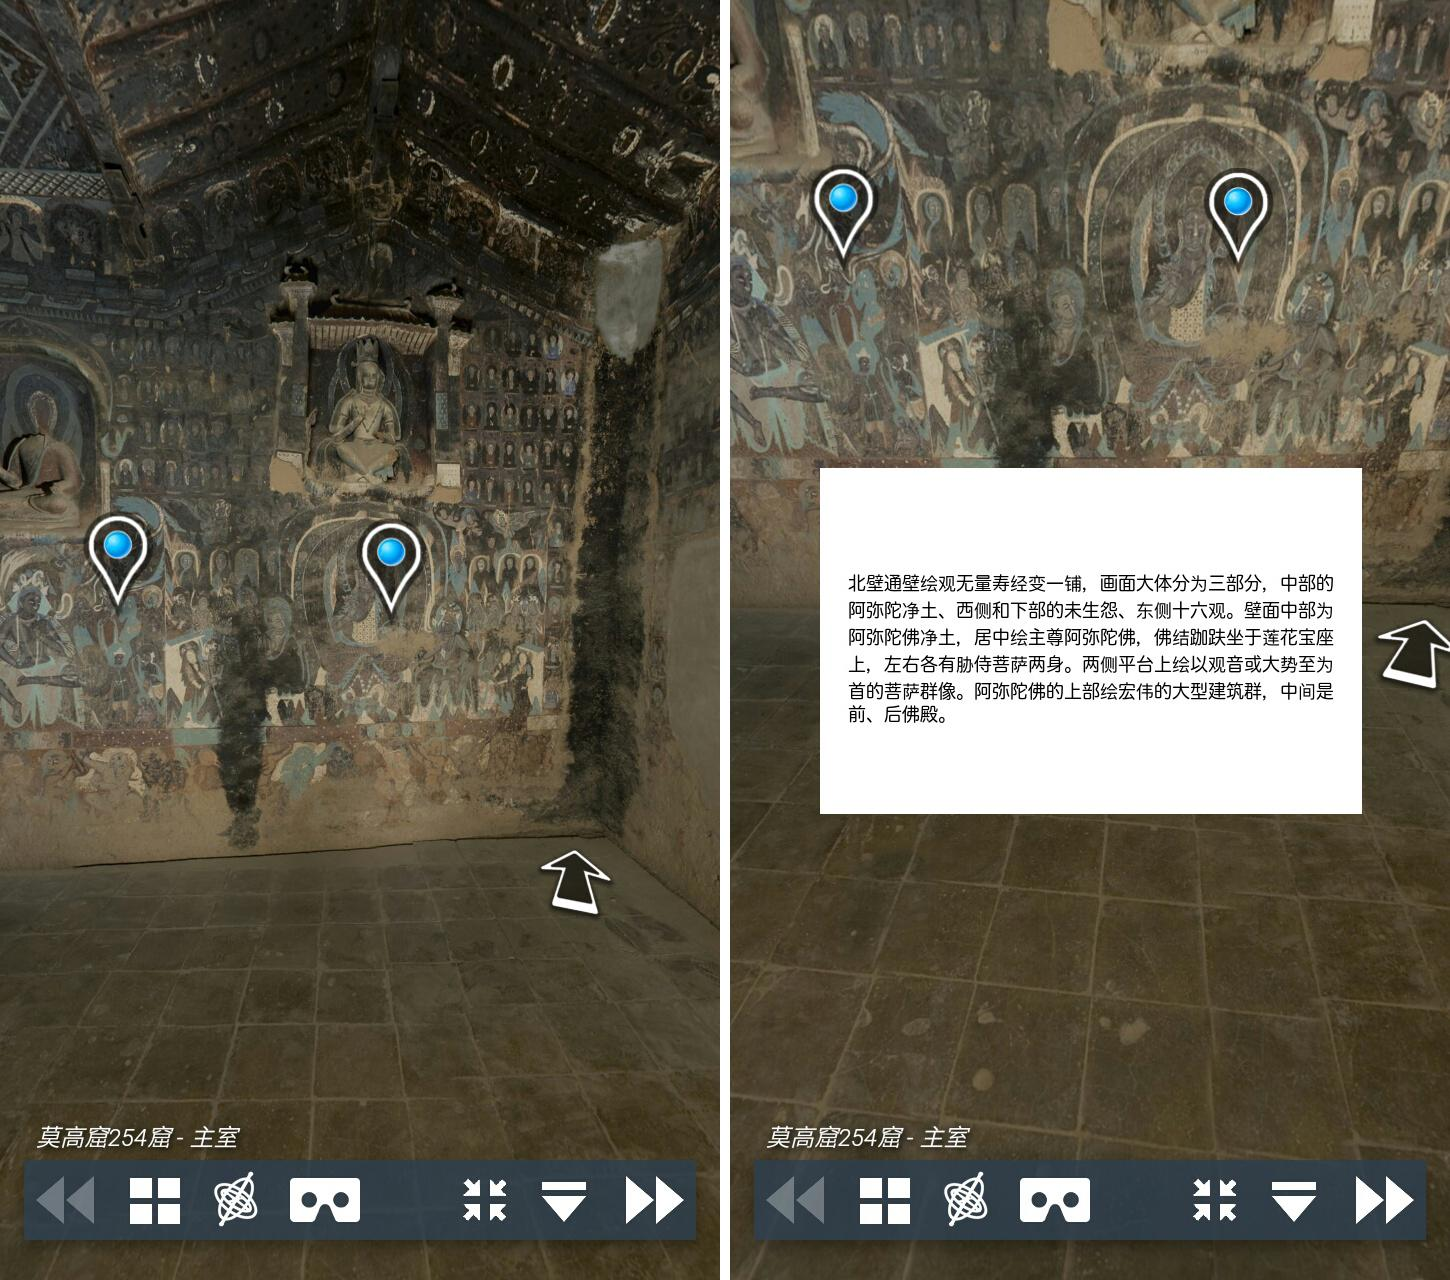
\includegraphics[width=.7\textwidth]{dunhuang}
}
\caption{全景漫游与景点介绍结合}
\label{fig:dunhuang}
\end{figure}

不可见的信息架构则包含用户输入的部分转换成特定的结构,例如用户的搜索功能等。这种信息架构有时也会影响前两者,比如通过自定义类别或提高相对信息权重来引导用户去关注某一类内容,这一点赋予了信息架构的设计管理者在设计制作完成后不断完善丰富交互内容的能力。

\subsection{信息架构组件}
信息架构的层次间可以互动,用户一般不常接触直接的层次,而是通过与信息架构组件间的交互完成信息互动。常见的组件有浏览帮手、搜索帮手、内容与任务,以及“不可见的”组件。

浏览帮手如网站的目录、导航栏、网站向导等,相当于文章的摘要和目录等,用以引导用户理解网站的大体结构。搜索帮手则是帮助带有特定目的浏览网站的用户更直接更快速地通过检索相关信息,直达自己所需信息的页面。内容和任务则是帮助带有探索目的的用户,以完成任务的形式去发现网站的功能,带有这种组件的网站一般为功能工具型网站而非展示类网站。“不可见的”组件即网站背后的算法和公式等,它们指导前台组件将用户导向更为合理高效的浏览途径上去。

在场景漫游中,内容与任务在场景内起主导作用,而在场景外则是导航与搜索起到引导用户踏足更多场景等作用。

\subsection{信息架构可视化}
信息架构不是藏在界面后面的东西,相反它出现在界面的各个角落。信息是一切操作的出发点和目的地,显然可见的信息架构有助于对此感兴趣的用户去进行深入体验。常见的信息架构的可视化体现在导航栏、搜索功能等上,但其他功能也会需要信息架构的支持,所以信息架构也被用来支持其他一切有功能的架构,以一种无形的形态在其他功能模块里实现自身的可视化。

\section{全景漫游的功能模型}
以功能目的为分类标准可讲全景漫游的功能分为:漫游功能、导航功能、搜索功能和记忆功能等。在实际应用中,功能的分块可因业务逻辑的复杂而增加或减少(如增添支付功能等)。以纯粹的体验角度而言,以上四项功能构成了用户在全景漫游中绝大部分的行为模式,故在此将它们列举出来讨论是较为合适的。

\subsection{漫游功能}
全景漫游,重在漫游。虽是全景漫游的绝对重点,但其实是设计中最不需要考虑的一点。因为对于该功能的使用,人完全是通过日常经验作出的本能反应,设计只能迎合这种需求。例如,想要让人可以观察到一个景点的全部景致就需要获取到这个地方的全景图(如图\ref{fig:hongcun}),而不是简单地提供一张平面图片去让用户想象。而要做到良好的全景漫游体验,只是提供一张全景图片是远远不够的,需要加入众多的场景互动,例如上文的点击热点展开景点的相关信息等。这部分功能可以用另一种全景体验来形容,称为“增强现实”。所谓“虚拟现实”,就是在模拟出全景场景后,再添加“增强现实”的元素,以达到以假乱真甚至超过现实一般的体验。

\begin{figure}[htp]
\centering
\fbox{
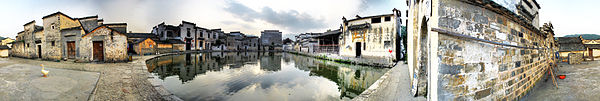
\includegraphics[width=.7\textwidth]{hongcun}
}
\caption{全景图像示例}
\label{fig:hongcun}
\end{figure}

\subsection{导航功能}
在场景间切换需要导航功能,这种导航与常见网站与手机应用内的导航基本类似\endnote{Fleming J. Web navigation: Designing the user experience[J]. Dux.typepad.com, 1998.},但因全景漫游的场景是空间形式的,而用户在其中并不能通过观察周围环境(虚拟场景中的地理信息通常是无效的,且脱离使用者真实所处的场景)分辨场景中的朝向,所以在场景内也通常会设置类似于一般游戏中的小地图\endnote{Flynn B M. Languages of navigation within computer games[C]// 2003:742.},如图\ref{fig:minimap}。这种地图主要起到定位使用者在虚拟场景内位置的作用,原因是真实世界内使用者的位移和转向与游戏中并不完全对应,且因全景漫游体验的封闭性,人很难找到一个参考物,而地图这种形式可以方便地指明场景中角色于其他物体间的参照关系。当使用者转向时,小地图上的代表角色的图标也会随之转向,通过仔细观察并反向演算可以恢复自身的朝向感。

\begin{figure}[htp]
\centering
\fbox{
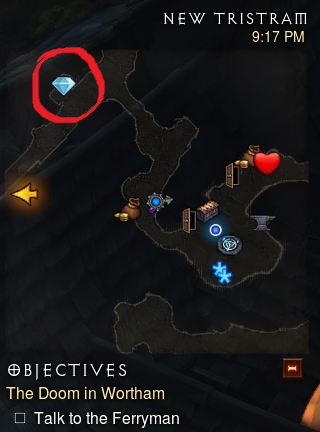
\includegraphics[width=.4\textwidth]{minimap}
}
\caption{一般游戏中的小地图}
\label{fig:minimap}
\end{figure}

\subsection{搜索功能}
搜索功能是非常常见的功能,在全景漫游中搜索功能与其他的基本类似,但因手部操作形式较为简单,故其输入文字信息的功能主要为语音识别来完成。同时,场景内的搜索功能可通过对物件的注视以获取悬浮提示的方式来选择搜索目标,即使用该物件作为搜索对象进行相关信息等检索。

\subsection{记忆功能}
记忆即储存相关信息,在探索行为中是非常重要的。记忆用户行为等目的不只是给予用户可查看的历史记录,更重要的是全景漫游中用户的操作目的性有时并不是那么明显,易造成误操作,通过还原场景功能可以撤销用户最近的若干次操作,同时可以保证场景漫游的流畅性。

系统记忆个人用户的身份信息也是有所必要的,因为每个人使用习惯与生理特性不同,系统应根据账号记忆不同账户用户的使用习惯及设置,从使用过程中自适应用户的操作,以减少用户进行复杂设置的需求。


\section{全景漫游的功能模块}
为了实现上述功能,需要在场景中插入很多组件。但组件的排序因遵循一定的规律,比如按照格式塔法则,人在注意一些相邻事物时会主动将相似的事物看作一个整体(即一个模块)进行考虑。在设计时即应按照模块化的思维对设计进行分类,模块的设计对于整个交互模式是极为重要的,好的模块设计有利于用户准确分辨并使用不同模块的功能。根据上文所述全景漫游的功能,可分为以下四个功能模块:
\begin{itemize}
	\item 导航功能模块
	\item 场景特殊模块
	\item 多输入交互模块
	\item 热点模块
\end{itemize}

\subsection{导航功能模块}
导航功能在场景漫游中使用频率并不高,主要是因为现今全景漫游大部分都只是小范围的活动,导航在整个场景漫游中起到的作用并不明显。但导航的不足会给用户带来迷茫和困惑,甚至令使用者不再愿意使用全景漫游。全景漫游力图给使用者每次带来的都是全新的历程,所以在探索新环境时,导航类的功能会给使用者提供一种情景和舒适感。

\subsubsection{导航的规则}
导航即是将东西整理并告知用户其所在位置的过程。导航的基本原则是在不影响清晰度和阅读效率的情形下展现尽可能多的信息层级结构,同时也需要指出用户当前所处的位置信息。导航除了基本的设计法则外,其规则基本遵循经验规则,如网站导航中经常采用的面包屑导航等。导航功能模块不是一个整体,通常情况下是是由一个主要的导航界面附带多个从属的局部导航功能模块所构成。优质的导航服务不会处处显露给用户其全部内容,而只是恰好在用户需要时能够在比较近的区域内找到所需的导航元素。

\subsubsection{导航的内容}
导航模块在不同场景下应该提供不同的内容。例如,主界面下就应当提供类别切换功能,而场景界面里应提供回到主屏幕的返回功能等。具体导航内容可见表\ref{tab:nav}。

\begin{table}[htbp]
\centering
\caption{界面导航内容}
\vskip 5pt
\begin{tabular}{lll}
\toprule
界面 & 导航内容 & 全局导航\\
\midrule
主界面 & 类别导航、搜索功能、本地内容、历史记录 & 否\\
类别 & 类别切换、场景列表 & 有 \\
搜索 & 无 & 有 \\
本地内容 & 类别切换、内容列表 & 有 \\
历史记录 & 类别切换、记录列表 & 有 \\
单个场景 & 场景内导航(小地图等) & 有 \\
\bottomrule
\end{tabular}
\label{tab:nav}
\end{table}

\subsection{场景特殊模块}
相比于普通页面的功能模块而言,场景的特殊模块需要额外考虑自身在屏幕内的适应性。例如一个悬浮在场景内的模块,需要在与场景其他部分重叠或接触时可被分辨并识别出来。模块的设计需要考量的因素相当之多,甚至到具体实施的阶段仍会不断调整模块间的适配性。关于模块定义的具体内容会在下一章内以实例的形式进行说明,本段只对一些基本的因素作出说明。

\subsubsection{模块的单义性}
单个模块不会出现歧义,但模块数量一旦超过一定规模,歧义现象就不可避免地出现了,表现为重复定义模块的部分或全部。当模块间所表现出的功能相近时,用户便会产生疑惑感继而不敢做出操作或是进行重复操作。例如,最常见的是签到功能中日历当日选项和“一键签到”的按钮,其功能意义相近,但点日历也许会有查看当日信息的操作可能,所以应该无论用户点击其中任意一项都可完成签到。在设计中应当尽可能避免这种容易迷惑用户的选项,而根据不同功能设置多个单义的功能模块,这样即方便使用者识别,也降低了开发过程中的代码耦合度\endnote{Huang C C, Kusiak A. Modularity in design of products and systems[J]. Systems Man \& Cybernetics Part A Systems \& Humans IEEE Transactions on, 1998, 28(28):66-77.}。

\subsubsection{模块的可组合性}
模块并不是独立存在的,模块间也会进行组合,表现为模块互相调用依赖等。比如,搜索模块也需要唤起语音输入模块来完成文本信息的录入,否则就失去了搜索的能力。同时,模块有时也会如队列般排列,比如重要操作都会需要二次验证,最简单的形式就是弹出一个确认框模块,只有用户选择了“确认”后才会继续完成后面的流程。


\subsection{多输入交互模块}
主要表现为语音输入模块、重力感应模块等。用户通过多种方式进行输入,设计时需要考量模块总输入的过滤筛选,并加以整合进行输出。

值得注意的是,全景漫游功能是建立在重力感应的技术基础上的,故最贴近其使用形式的交互模式可以采用摆动头部这类动作的形式。可以通过实验方式采集每种基础头部动作的三维运动加速度,经过预处理后作为头部动作的特征量,然后通过建立隐含马尔可夫模型后对实际运用过程中采集的头部动作数据进行识别,转化为基础头部动作的序列,达到头部动作实现交互操作的功能\endnote{孔俊其. 基于三维加速度传感器的手势识别及交互模型研究[D].苏州大学,2009.}。

\subsection{热点模块}
场景中有很多非通用但也具有交互能力的模块,统一将其设计称为一个触发器,当用户选择后便给它发出一个激活信号,令其执行预定的操作。热点模块类似于生活中电器的开关,随处可见非常普通但也很重要。

\section{全景漫游的信息架构小结}
全景漫游系统中信息架构是以真实世界的游乐场为类比对象、自顶向下为主要组织形式、其他架构为辅助的多层次、多路径的信息组织方式。用户进行漫游时以漫游功能为目标、导航功能为导向进行信息浏览,并针对用户使用习惯定义例如多输入交互模块和热点模块等特殊模块以方便交互操作。全景漫游系统中主体模块为导航模块,其不仅仅体现在导航界面的展示,更是整体应用中处处可见的导航功能背后的架构。用户通过实际交互操作的过程,其本质就是与以导航功能为核心的信息架构进行信息交互的过程,漫游功能则是距离用户最近的模块,承担了交互的界面作用。

本章从信息架构阐述了全景漫游系统的信息模型,认识到信息架构的优劣是全景漫游体验的根本因素,提出了全景漫游系统中漫游是以信息发现(即导航)为导向的信息交互的观点。既往全景漫游中应用以单个场景为主导,着重于用户“即来即用、用完即走”的漫游体验,忽视了用户的留存行为是于用户对信息可达性的高标准要求的实际体现。而上述研究中指出,用户对信息的需求对信息的组织形式有较高的要求,故符合用户心理预期的信息架构是能够从功能上满足用户对信息获取便捷性和高效性的需求,是全景漫游设计的必要内容。